\urldef{\persianwordlist}\url{http://github.com/reza1615/PersianOcr}

As mentioned before, the methods used in this work for facing the CL-WSD problem, exploit the use of a monolingual corpora together with a bilingual lexicon. In the following, first we describe the data acquisition and preparation process for these resources in Persian. Then, we evaluate two baselines on the created Persian CL-WSD benchmark, described in Section~\ref{sec:persian_collection}: the first is the standard baseline introduced in the SemEval 2013 CL-WSD task~\cite{lefever2013semeval} and the second is a state-of-the-art system called CO-Graph~\cite{duqueco}. Finally, we evaluate our approach, introduced in Section~\ref{sec:methodology}, and compare it with the baselines.

\vspace{-0.2cm}
\subsection{Data Preparation}

As discussed in Section~\ref{sec:relatedwork}, we selected the Hamshahri collection for the required monolingual corpora. We first normalized the collection using Lucene's PersianNormalizationFilter. After normalization, by comparing the tokens in the collection with a comprehensive list of Persian words\footnote{\persianwordlist}, we observed that from approximately 587K distinct tokens in the collection only 94K(16\%) are in the list of the known words. Tracing the collection's tokens, we observed many incorrect tokens, create by concatenation of two words. For example ``\<drketAb>'' (``inbook'') should have been split in two words: ``\<dr ketAb>'' (``in book'').% The list contains the words in the Dehkhoda and Moin Dictionary, Open Office's Persian spell checker, and the title of Persian pages in Wikipedia.

In order to mitigate this problem, we implemented a greedy decompounder which splits a token in at most two parts. The decompounder uses an existing word-frequency list to find the best splitting alternative. We create this word-frequency list from the Hamshahri collection with the assumption that the words with the higher frequencies in the collection are more probable to be correct. The decompounder first finds all the possible alternatives for splitting the word and uses the list to compute the mean value of the frequencies of the two new tokens. Then, it splits the token if the mean value is higher than the frequency of the original token.

In order to increase the accuracy of the decompounder and avoid incorrectly splitting the words, we randomly selected 500 cases from all the split ones and checked whether they had correctly been decompounded. 
%most the problems come from name entities or persian-written words from other languages as well as incorrect words probably come from errors in OCR. 
After the evaluation, we observed an error rate of 32\%. In order to decrease this error rate, %value of This decision is only based on the value of Harmonic Mean
we applied an AD Tree classifier together with 10-Fold Cross Validation while using the geometric mean, harmonic mean, and standard variation of the frequencies of the split words as the features. The classifier achieved a precision of 0.81. Table \ref{table:confusionmatrix} shows that the error rate of the system has been reduced to 7.6\% (FP/P) as it only decompounds 55\% (P/All) of the introduced candidates\footnote{The decompounder source code is available at software/decompounder}.

\begin{table}[t!]
\begin{center}
\caption{The confusion matrix of 500 annotated tokens after decompounding using AD Tree classifier. } 
\vspace{-0.2cm}
\begin{tabular}{c c c c }
\hline
 & & \multicolumn{2}{c}{Predicted} \\
 & & Yes & No \\
\hline
\parbox[t]{2mm}{\multirow{2}{*}{\rotatebox[origin=c]{90}{Actual~~}}} & Yes & 254 (TP) & 84 (FN) \\[1ex]
 & No & 21 (FP) & 141 (TN)\\[1ex]
\hline
 &  & 275 (P) & 225 (N)\\
\label{table:confusionmatrix} 
\end{tabular}
\end{center}
\vspace{-1.3cm}
\end{table}

Having the designed decompounder, we applied it on the all 587K unique tokens of the collection. While the decompounder split about 132K tokens, the number of unique words in the collection decreased from 587K to 485K, of which 213K(43\%) were known by the Persian's words list. Therefore, using the decompounder, we increased the number of the known words  269\% (from 94K to 213K) while introducing approximately 7.6\% error in the split tokens\footnote{The Zipf's distribution of the processed Hamshahri and ANC collections is available at supplementary-materials/zipf}.

Beside the monolingual corpus, a bilingual lexicon is required for our unsupervised CL-WSD approach. %As it is discussed in Duque et al.~\shortcite{duque2015choosing}, the choose of the lexica play an important role in unsupervised systems. In the existence of parallel corpora, they are used to create the bilingual lexica~\cite{duqueco,lefever2013semeval}. 
While using  parallel corpora is considered as a more effective method for creating  lexica~\cite{duque2015choosing}, due to the lack of reliable parallel corpora, we directly extracted the data from Google Translate. Beside the provided translation, the online platform also provides the rate indicating how often the translation is used regarding to its corresponding word in the source language. In our lexicon, this translation probability rate can have one of the three values of 0.25 (rare), 0.5 (uncommon), or 0.75 (common)\footnote{Available at resources/dictionary}. 

\vspace{-0.2cm}
\subsection{Baselines}
In this section, we explain two baselines for the created Persian CL-WSD benchmark. These baselines are further compared with the results of our approach.

The first one---the \emph{Standard} baseline---follows the method introduced in the SemEval 2013 CL-WSD task for creating the baseline. Similar to the task, for the \emph{Best Result} and \emph{Out-Of-Five} evaluations, we selected the most common and the five most common translations respectively. %If there exists more than the required translations in an specific popularity rate group, we randomly selected the required ones from the group.
Evaluating the baselines on the Persian CL-WSD task using F-measure evaluation measure, we observed the value of 15.8 for the \emph{Best Result} and 41.8 for the \emph{Out-Of-Five} evaluation\footnote{Available at resources/baseline}. 

Since the standard baseline considers only the most common translations, it cannot provide a realistic view on the effectiveness of the CL-WSD systems. Therefore, we evaluate the created Persian benchmark on the state-of-the-art unsupervised CL-WSD system called CO-Graph~\cite{duqueco}. The CO-Graph system offers competitive results in the SemEval 2010 and SemEval 2013 CL-WSD tasks, for all the proposed languages, namely Spanish, French, Italian, Dutch and German. It is able to outperform all of the unsupervised participating systems using only monolingual corpora, and even most of the ones which use parallel corpora or knowledge resources.

The initial hypothesis for the CO-Graph system relies on the idea that words in a document tend to (statistically) adopt a related sense. The system first creates a graph of connections between the words, using the documents in the collection, and then applies different algorithms (Dijkstra, Community-based, Static PageRank, Personalized PageRank) to disambiguate the words based on their contexts. The construction of the graph is based on the statistical significance (p-value) of the co-occurrences of the words in the same documents (more details in Duque et al.~\shortcite{duqueco}). % such that the probability distribution that models the co-occurrences of two words inside the same document, given a specific number of documents, is compared against a null model that represents what could be considered co-occurrence by pure chance. If the significance of the co-occurrence is above a given threshold, both words will be connected by an edge in the resulting graph (more details in Duque et al.~\shortcite{duqueco}).
%community-based algorithms and Dijkstra's algorithm) and those which only take into account the structure of the graph (PageRank algorithm). Each algorithm uses the context words for performing the disambiguation in a different way.
%: the probability distribution that models the co-occurrences of two words inside the same document, given a specific number of documents, is compared against a null model that represents what could be considered co-occurrence by pure chance. 
%If the significance of the co-occurrence is above a given threshold, both words will be connected by an edge in the resulting graph.
%The initial hypothesis for the CO-Graph system relies on the idea of consistency inside a document, this is, a document is a coherent piece of information, so we can assume that words in a document tend to (statistically) adopt a related sense. We consider that two words frequently appearing in the same document share some kind of semantic information that points to a related sense, and must be connected by an edge in a graph. Hence, the main pre-requisite behind the CO-Graph system is the availability of a corpus divided into documents, each one of them related to a specific subject or topic. Since the co-occurrence of two words inside a document may not guarantee by itself that they share a common sense, the construction of the graph is based on the statistical significance of those co-occurrences: the probability distribution that models the co-occurrences of twowords inside the same document, given a specific number of documents, is compared against a null model that represents what could be considered co-occurrence by pure chance. If the significance of the co-occurrence is above a given threshold, both words will be connected by an edge in the resulting graph.
%Regarding the specific Cross-Lingual Word Sense Disambiguation (CLWSD) tasks, once that we build the co-occurrence graph for a specific language, we need an algorithm that processes the information about the target word (mainly, its context) for exploring the graph and extracting the most probable translation of that word. We have explored two types of algorithms: those which make use of the weights in the co-occurrence graphs (community-based algorithms and Dijkstra's algorithm) and those which only take into account the structure of the graph (PageRank algorithm). Each algorithm uses the context words for performing the disambiguation in a different way. The community-based algorithms find subgraphs (communities) inside the initial graph, and then search for those communities containing translations of the target word which are closer to those containing translations of the context words. The technique based on Dijkstra's algorithm (CITE) compute those distances directly over the initial words of the graph, for finding those translations of the target word more influenced by context words, as it is explained later on. Finally, the technique based on the PageRank algorithm (CITE) gives importance to the translations of context words by assigning them an initial weight at the beggining of the algorithm. This weight will then spread along the graph, and the translation of the target word with highest PageRank score will be selected.
%The base of knowledge used for performing CLWSD in the Persian language is different that the one used in the SemEval CLWSD tasks. However, the Persian corpus is created from documents, each one of them representing a specific piece of news or article inside a newspaper. Therefore, we consider that the hypothesis for the creation of the co-occurrence graph is fulfilled, since each document is likely to be related to a unique topic. 
%It is important to notice that the total number of nouns that can be present in the graph is around 68,000 (although the real number of words used in the graph will depend on the threshold of the p-value). Languages that obtain better results tend to have graphs with less words ($\sim$ 25,000 in French, $\sim$ 43,000 in Spanish, and $\sim$ 54,000 in Italian), while languages for which the task is more difficult present many more possible nouns in the graphs ($\sim$ 125,000 for German and $\sim$ 169,000 for Dutch).
%The technique that has offered the most stable results in the experiments is the one based on Dijkstra's algorithm. This technique is focused on extracting the influence that each word of the context has on each of the possible translations of the target word, by considering the weighted distance between them. Since a weight of a link between two words in the graph represents the significance of that co-occurrence, we have to consider the inverse of that weight as a measure of the distance between those two nodes. Then, Dijsktra's algorithm is run for finding the shortest paths between each translation of a context word and each translation of the target word. Once that we have those paths, we can weight the influence of a context word over a translation, as the sum of the original weights of the edges in the path, divided by the total number of edges. Finally, the weight assigned to each possible translation is the highest weight (influence) given by a context word.
%Regarding the results obtained by the technique based on Dijkstra's algorithm, we can conclude that the weights assigned to the links in the process of building the co-occurrence graph are useful for determining the influence of the context words on the target word.

In order to evaluate the CO-Graph system on the Persian benchmark, we first created the graph using the articles of the Hamshahri collection, each as a document. In the construction of the graph, we only took into account the nouns by POS tagging and parsing the collection using TagPer~\cite{seraji2012} and PerStem~\cite{dehdari2008link} tools. The process of creating the graph took approximately 34 hours. We then evaluated the benchmark using the described lexica and all four algorithms with the p-value range of $10^{-5}$ to $10^{-17}$. Finally, we found Dijkstra algorithm together with p-value=$10^{-6}$ as the best performing approach with the F-measure metrics of 17.4 for the \emph{Best Result} and 44.1 for the \emph{Out-Of-Five} evaluation\footnote{The detailed results are available at supplementary-materials/co-graph}. %Regarding to the experiments on the five other languages in the SemEval 2010 and 2013 CL-WSD task, the best and the most stable results were achieved using  for creating the graph. 
%In order to verify our assumptions on selecting the Dijkstra algorithm as well $p=10^{-6}$, . As the results are shown in Figure~\ref{figure:cograph-best} and Figure~\ref{figure:cograph-best}, we observe that the results in Persian are quite similar to the other tested languages, such that the Dijkstra algorithm on $p=10^{-6}$ shows the best results .

\vspace{-0.2cm}
\subsection{Evaluation}

\begin{table}[t!]
\begin{center}
\caption{Results of F-measure on \emph{Out-Of-Five (OOF)} and \emph{Best Result (Best)} evaluations based on RelAgg and RelGreedy approaches. The vector representations of words were created by the Word2Vec~\cite{mikolov2013efficient} and GloVe~\cite{pennington2014glove} methods with 50 and 200 dimensions, using the corpus of the Hamshahri collection} 
\vspace{-0.2cm}
\begin{tabular}{c c l c }
\hline
Eval. & Method & Vector Repres. & F-measure \\
\hline

\multirow{10}{*}{OOF} & \multirow{4}{*}{RelAgg} & W2V-200 & 50.2 \\
& & W2V-50 & 49.9 \\
& & GloVe-200 & \textbf{50.3} \\
& & GloVe-50 & 49.7 \\
\cline{3-4}
& \multirow{4}{*}{RelGreedy} & W2V-200 & 49.3 \\
& & W2V-50 &  49.5 \\
& & GloVe-200 & 50.2 \\
& & GloVe-50 & 50.0 \\
\cline{2-4}
& \multicolumn{2}{c}{CO-Graph Dijkstra} & 44.1\\
& \multicolumn{2}{c}{Standard Baseline} & 41.8\\
\hline
\hline
\multirow{10}{*}{Best} & \multirow{4}{*}{RelAgg} & W2V-200 & 18.8 \\
& & W2V-50 & 18.3 \\
& & GloVe-200 & \textbf{19.8} \\
& & GloVe-50 & 18.2 \\
\cline{3-4}
& \multirow{4}{*}{RelGreedy} & W2V-200 & 18.3 \\
& & W2V-50 &  18.4 \\
& & GloVe-200 & 18.5 \\
& & GloVe-50 & 18.4 \\
\cline{2-4}
& \multicolumn{2}{c}{CO-Graph Dijkstra} & 17.4\\
& \multicolumn{2}{c}{Standard Baseline} & 15.8\\
\hline
\label{table:results} 
\end{tabular}
\end{center}
\vspace{-1.0cm}
\end{table}

In this section, we report the evaluation of our approach on the Persian benchmark and compare it with the baselines. In the first step, given the corpus of the processed Hamshahri collection, we created semantic vector representations of the words in Persian using two state-of-the-art methods: Word2Vec~\cite{mikolov2013efficient} and GloVe~\cite{pennington2014glove}. We trained the Word2Vec model using its toolkit\footnote{\url{https://code.google.com/p/word2vec}} by applying the Skip-Gram approach with sub-sampling at $t=10^{-4}$. The GloVe word representation was also constructed by its toolkit\footnote{\url{http://nlp.stanford.edu/projects/glove}} while using its default parameter settings. Regarding the common parameters, we selected the context windows of 5 words, epochs of 25, and words count threshold of 5 (the words with collection frequency less than five are considered as noise and filtered out) for both methods. Using 40 threads, the construction of each model took approximately 45 minutes for Word2Vec, and less than 20 minutes for GloVe. For each method, we prepared a set of three models with vector dimensionalities of 50, 100, and 200.

In the next step, we applied POS tagging on the sentences of the SemEval 2013 CL-WSD task and only selected the verbs and nouns as the context of the ambiguous words. We then lemmatized the words using WordNetLemmatizer of the NLTK toolkit and found their translations in the  bilingual lexicon. Using the vector representations of the translated words, we calculated the relatedness score of each translation candidate to its context using RelAgg and RelGreedy (Section~\ref{sec:methodology}). The translation probability rate in our lexica was used as the $P(t)$ value in Eq.~\ref{formula:relagg} and Eq.~\ref{formula:relgreedy}. Given the score of the translation candidates, we created the run files for the \emph{Out-Of-Five} evaluation by selecting the 5 best translations, and the top one for the runs of the \emph{Best Result} evaluation. Table~\ref{table:results} shows the \emph{Out-Of-Five} and \emph{Best Result} evaluation results of RelAgg and RelGreedy relatedness approaches together with Word2Vec's and GloVe's vector representations of words each with 50 and 200 dimensions on the Persian CL-WSD benchmark using the F-measure metrics. The results for dimensionality 100 were very similar to those of 50 and are not reported here for space considerations.%\footnote{http://www.nltk.org}

\begin{figure}[t!]
  \centering
    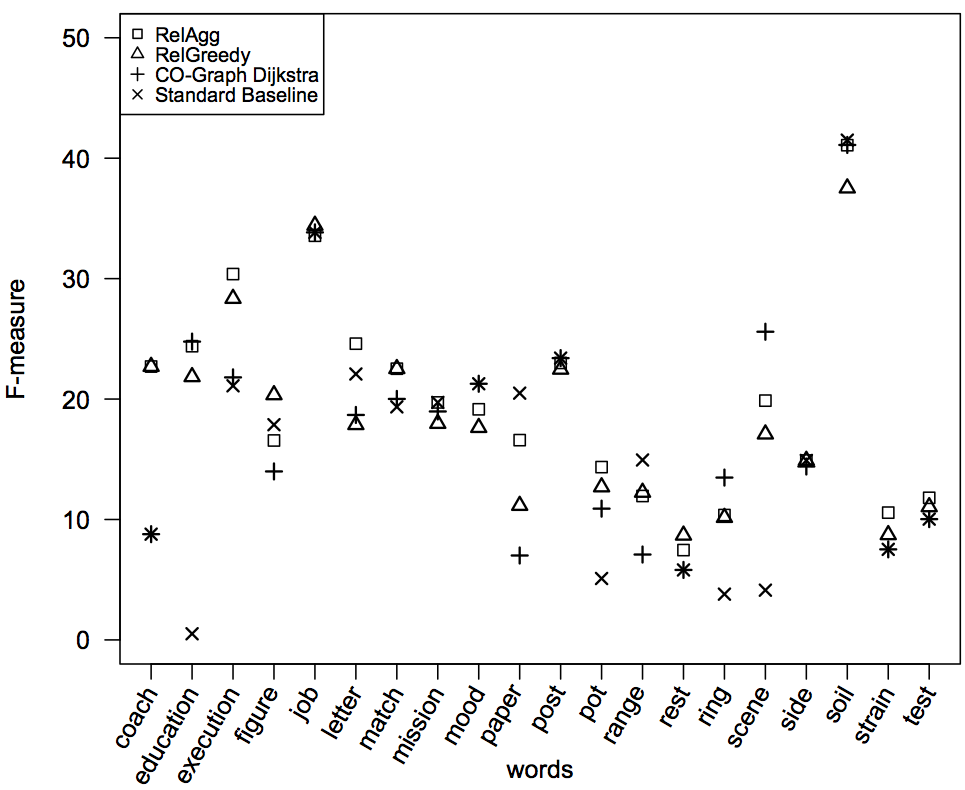
\includegraphics[width=0.5\textwidth]{plots/word-based-oof.png}
  \caption{Results of the \emph{OOF Result} evaluation based on each word using F-measure}
  \label{figure:wordresults-oof} 
\vspace{-0.7cm}
\end{figure}

The results for both the \emph{Out-Of-Five} and \emph{Best Result} evaluations show that our approach based on vector representation of the words outperforms the standard as well as the CO-Graph baselines. Comparing the relatedness approaches, we observe similar results for the RelAgg and RelGreedy methods, while RelAgg has slightly better performance, specially in the \emph{Best Result} evaluation. Regarding the different vector representations of the words with common evaluation and relatedness methods, we also see very similar results, while the GloVe method with 200 dimensions shows overall better performance.

In order to observe the effectiveness of the systems on different words, we selected the best performing settings in both RelAgg and RelGreedy (GloVe with 200 dimensions), and compared them with the standard and the CO-Graph baselines. The results for the \emph{Out-Of-Five} evaluation are shown in Figure~\ref{figure:wordresults-oof}\footnote{The corresponding plot for the \emph{Best Result} is available at supplementary-materials/evaluation}.

The results show that while for most words our approach outperforms the standard baseline as well as the CO-Graph system, none of the systems could outperform the standard baseline for ``mood'' and ``side''. Analyzing the evaluation results of these words, we observed that in some sentences, none of the nouns and verbs in the context share any common topic with senses of the ambiguous term. For example, using only the semantics of the nouns and verbs in the context, the correct sense of ``mood'' cannot be distinguished in either of the sentences: ``it reflected the \textit{mood} of the moment'' (state of the feeling) and ``a general \textit{mood} in Whitehall'' (inclination, tendency) . Similar cases were observed for the word ``side'': e.g., ``both \textit{sides} reaffirmed their commitment'' (groups opposing each other) in comparison to ``at the  \textit{side} of the cottage'' (a position to the left or right of a place). These examples show the limitations of the context-based methods. In addition to the context, the probability of occurrence of the words in a specific order (language modeling), potentially including terms of closed POS classes, is probably the missing piece here. 
